\chapter{Results and Analysis}
\label{chapter:results}

\section{Acceleration of Post-Quantum Key Encapsulation Mechanisms}

\todo[inline]{
What specialized instructions and features applicable for post-quantum keyencapsulationmechanisms are available in z15 and how are they used in context?
}

This section studies the \gls{nist} submissions' underlying mathematics, the authors' own optimizations as well as relevant literature on cryptography optimization.

\subsection{Identifying Hot Paths}
\label{section:results:hot-paths}

The following sections analyzes the \gls{ntru} and \gls{mceliece} submissions to the \gls{nist} standardization process, in terms of the reference implementations and what branches the code takes, how many times they are taken, as well as how many instructions are retired in each function. Unless otherwise stated, the measurements are the percentage of instructions performed in a function or in a line of code, relative to the parent.

All of the data as well as further visualizations not included in this work is published on GitHub\footnote{\href{https://github.com/profiling-pqc-kem-thesis/data}{https://github.com/profiling-pqc-kem-thesis/data}}.

\subsubsection{NTRU}

The \gls{ntru} reference implementations consists of three API methods - keypair generation via \textit{crypto\_kem\_keypair}, encryption (encapsulation) via \textit{crypto\_kem\_enc} and decryption (decapsulation) via \textit{crypto\_kem\_dec}  decryption (decapsulation). These API functions may in turn call several internal functions, such as the polynomial math library which functions are prefixed \textit{poly\_}.

The following graphs contain relative measurements denoting the percentage of instructions spent in each method. Both the HPS and HRSS variants of \gls{ntru} perform alike, hence only one set of graphs is shown for \gls{ntru} as a whole.

Figure \ref{figure:result:hot-paths:ntru:crypto_kem_keypair} shows us that $40\%$ of the instructions of generating a key-pair is spent in the library function \textit{poly\_Rq\_mul} - a function which multiplies two polynomials in $\mathbb{R}^q$. Another $20\%$ of the instructions are spent on inverting a polynomial in $\mathbb{R}^2$ - in \textit{poly\_R2\_inv}. In total, the polynomial math accounts for at least $60\%$ of the time spent on generating a keypair.

\begin{figure}[H]
    \centering
    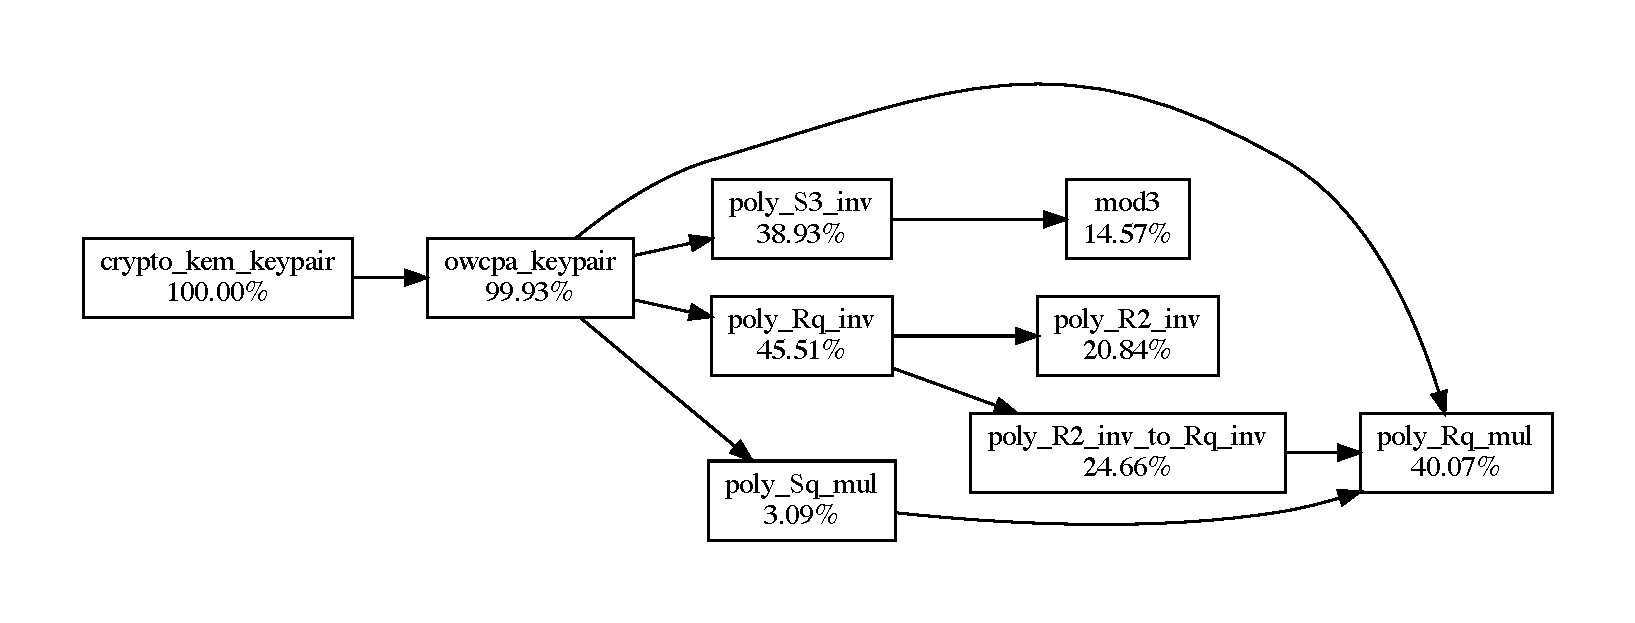
\includegraphics[width=15cm, height=10cm, keepaspectratio]{chapters/results/hot-paths/ntru/crypto_kem_keypair.pdf}
    \caption{Relative instruction count of \gls{ntru}'s \textit{crypto\_kem\_keypair}}
    \label{figure:result:hot-paths:ntru:crypto_kem_keypair}
\end{figure}

Figure \ref{figure:result:hot-paths:ntru:crypto_kem_enc} describes the encapsulation API function. The key is generated using random bytes which are fed through 256-bit \gls{aes} in its Electronic Code Book (ECB) configuration to produce uniformly random bytes. Again, we see a significant percentage of the instructions spent in the polynomial library - in \textit{poly\_Rq\_mul}.

\begin{figure}[H]
    \centering
    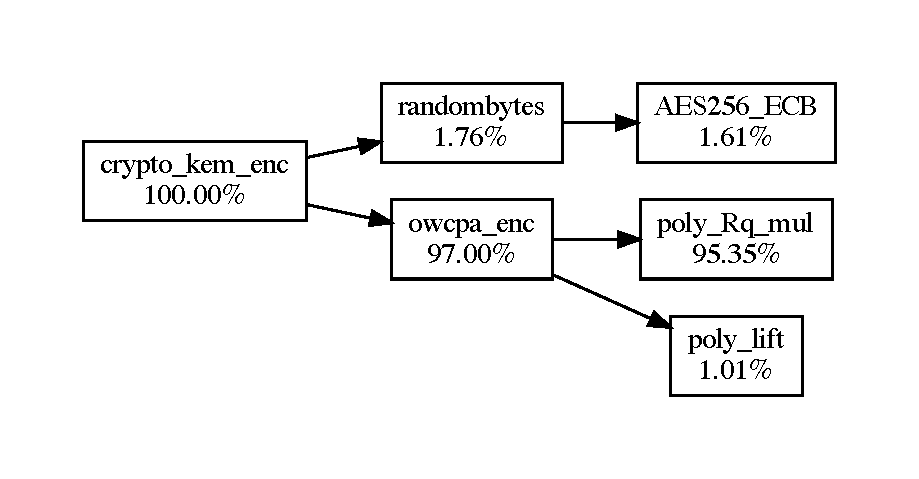
\includegraphics[width=15cm, height=10cm, keepaspectratio]{chapters/results/hot-paths/ntru/crypto_kem_enc.pdf}
    \caption{Relative instruction count of \gls{ntru}'s \textit{crypto\_kem\_keypair}}
    \label{figure:result:hot-paths:ntru:crypto_kem_enc}
\end{figure}

The decryption function of \gls{ntru} is presented in figure \ref{figure:result:hot-paths:ntru:crypto_kem_dec}. Virtually all of the instructions spent decrypting (decapsulating) a key is spent in the \textit{poly\_Rq\_mul} function.

\begin{figure}[H]
    \centering
    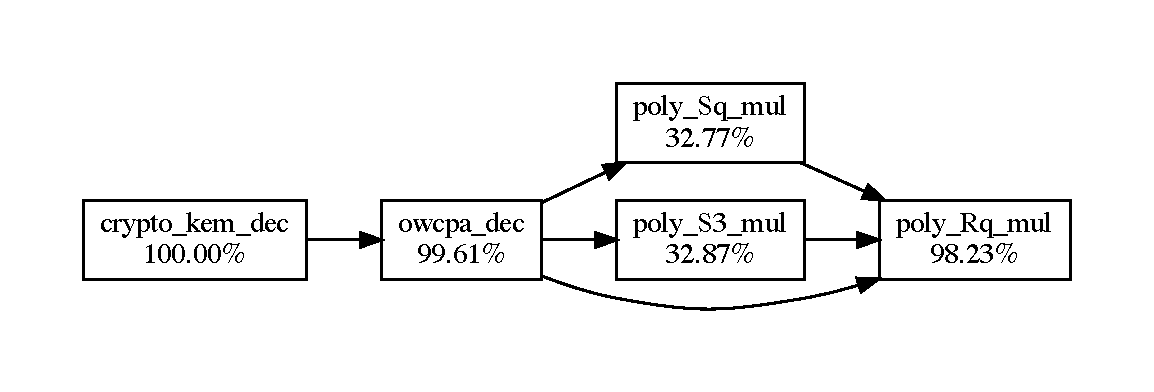
\includegraphics[width=15cm, height=10cm, keepaspectratio]{chapters/results/hot-paths/ntru/crypto_kem_dec.pdf}
    \caption{Relative instruction count of \gls{ntru}'s \textit{crypto\_kem\_dec}}
    \label{figure:result:hot-paths:ntru:crypto_kem_dec}
\end{figure}

Looking at the code of \textit{poly\_Rq\_mul} as shown in figure \ref{figure:result:hot-paths:ntru:poly_Rq_mul}, it is evident that the vast majority of instructions are spent on multiplying and adding numbers in loops. The value of \textit{NTRU\_N} corresponds to the parameter set. For \gls{ntru} HRSS 701, the value is 701 and for \gls{ntru} HPS 4096821 the value is 821.

\begin{figure}[H]
    \centering
    \begin{lstlisting}[language=C]
void poly_Rq_mul(poly *r, const poly *a, const poly *b) {
  int k, i;

  for (k = 0; k < NTRU_N; k++) {
    r->coeffs[k] = 0;
    for (i = 1; i < NTRU_N - k; i++) // 10.21%
      r->coeffs[k] += a->coeffs[k + i] * b->coeffs[NTRU_N - i]; // 42.75%
    for (i = 0; i < k + 1; i++) // 8.20%
      r->coeffs[k] += a->coeffs[k - i] * b->coeffs[i]; // 38.79%
  }
}
    \end{lstlisting}
    \caption{Annotated source code of \gls{ntru}'s \textit{poly\_Rq\_mul}}
    \label{figure:result:hot-paths:ntru:poly_Rq_mul}
\end{figure}

To summarize, it is shown that factors such as the speed of \gls{aes} has little to do with the overall performance of the algorithm. Furthermore, it seems as if the polynomial library functions account for the vast majority of instructions spent on key-pair generation, encryption and decryption. The function \textit{poly\_Rq\_mul}, which multiplies two polynomials in $\mathbb{R}^q$), accounts for most of the calculations performed.

\subsubsection{Classic McEliece}
The \gls{mceliece} reference implementation consists of three API methods - \textit{crypto\_kem\_keypair}, \textit{crypto\_kem\_enc} and \textit{crypto\_kem\_dec} for key-pair generation, encryption (encapsulation) and decryption (decapsulation), respectively. These API functions may in turn call several internal functions. We will only present the hot-paths for the \gls{mceliece} 8192128 non-f variant because it can quite accurately represent the hot-paths for all \gls{mceliece} variants. In the appendix, all hot-paths can be found. 

In figure \ref{figure:result:hot-paths:classic-mceliece:crypto_kem_keypair}, we can see the \textit{crypto\_kem\_keypair} function and its only significant internal function, the \textit{pk\_gen} function that takes up 98.57\% of the execution time. In figure \ref{figure:result:hot-paths:classic-mceliece:pk_gen}, we can see the deeper look into the \textit{pk\_gen} function there we can see that all its internal functions and that they do not make up much of the instructions. Most of the instructions are inside of the \textit{pk\_gen} function itself.\todo{explain better}

\begin{figure}[H]
    \centering
    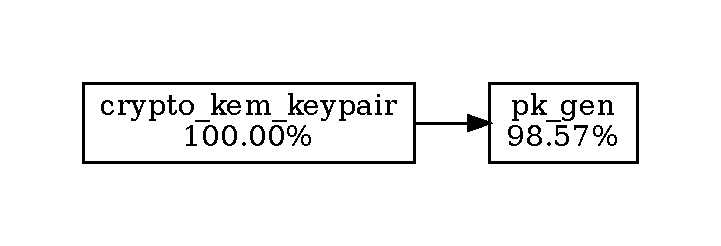
\includegraphics[width=15cm, height=10cm, keepaspectratio]{chapters/results/hot-paths/classic-mceliece/8192128/crypto_kem_keypair.pdf}
    \caption{Relative instruction count of \gls{mceliece}'s \textit{crypto\_kem\_keypair}}
    \label{figure:result:hot-paths:classic-mceliece:crypto_kem_keypair}
\end{figure}

\begin{figure}[H]
    \centering
    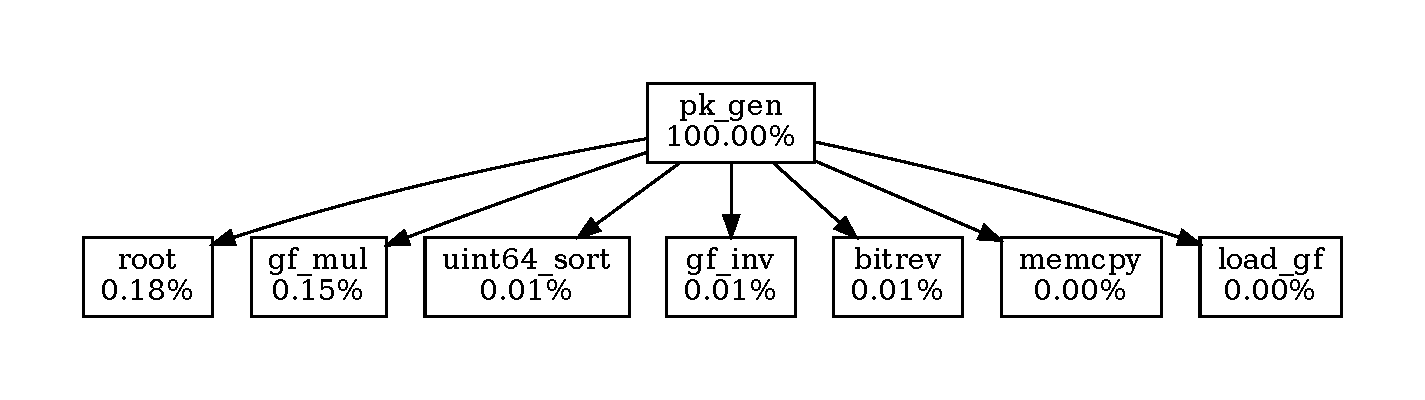
\includegraphics[width=15cm, height=10cm, keepaspectratio]{chapters/results/hot-paths/classic-mceliece/8192128/pk_gen.pdf}
    \caption{Relative instruction count of \gls{mceliece}'s \textit{pk\_gen}}
    \label{figure:result:hot-paths:classic-mceliece:pk_gen}
\end{figure}

\begin{figure}[H]
    \centering
    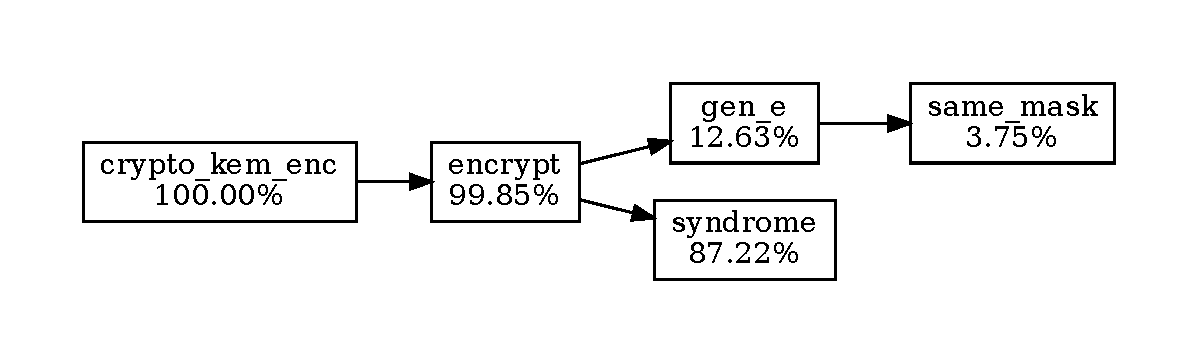
\includegraphics[width=15cm, height=10cm, keepaspectratio]{chapters/results/hot-paths/classic-mceliece/8192128/crypto_kem_enc.pdf}
    \caption{Relative instruction count of \gls{mceliece}'s \textit{crypto\_kem\_keypair}}
    \label{figure:result:hot-paths:classic-mceliece:crypto_kem_enc}
\end{figure}

\begin{figure}[H]
    \centering
    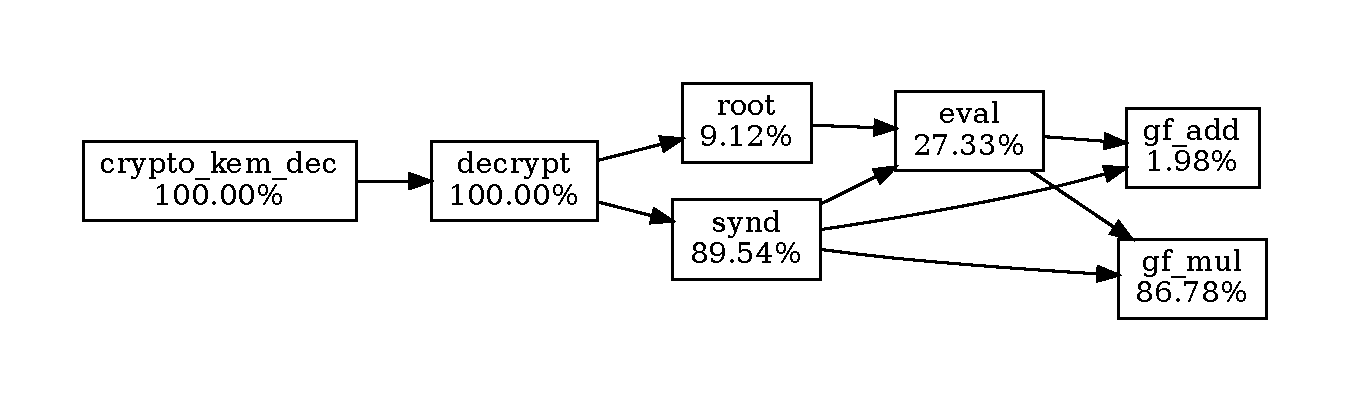
\includegraphics[width=15cm, height=10cm, keepaspectratio]{chapters/results/hot-paths/classic-mceliece/8192128/crypto_kem_dec.pdf}
    \caption{Relative instruction count of \gls{mceliece}'s \textit{crypto\_kem\_dec}}
    \label{figure:result:hot-paths:classic-mceliece:crypto_kem_dec}
\end{figure}

\todo[inline]{Var tydliga med hot paths och tid. Exempelvis så lär diagrammet för pk\_gen visa 0\% för vissa funktioner så som root, men om vi ser till hot paths så lär vi se att de kallas flera miljoner gånger. Kanske ha en graf som visar antalet invocations?}

\todo[inline]{Ingen microbenchmark för eval, gf\_mul och gf\_add - de körs så många gånger att overheaden för profiling blev 1000x. McEliece kallar på många många tusen funktioner (hundra tusen, uppemot miljoner?) - det i sig bör ge mer overhead. }

\section{Post-Quantum Cryptography on z15}

\todo[inline]{
What specialized instructions and features applicable for post-quantum keyencapsulation mechanisms are available in z15 and how are they used in context?

Litteraturstudien.
}

\section{The Performance of Post-Quantum Key Exchange Mechanisms}

This section presents the results of the experiment as outlined in section \ref{section:method:experiment}. It further discusses the performance of \gls{post-quantum} \glspl{kem} and how they may differ on various architectures and hardware.

\subsection{Algorithm Performance}

In section \ref{section:method:experiment:phase1:implementation-configurations} it was written that the monitored functions for the micro benchmark would be based off of data found in the hot paths analysis. In the end, the functions presented in Table \ref{table:results:performance:micro-functions} were monitored during the micro benchmark. Note that although the randombytes function is available in both \gls{ntru} and \gls{mceliece}, it was found in section \ref{section:results:hot-paths} to not be significant enough to warrant further analysis.

\begin{table}[H]
    \centering
    \caption{Monitored Functions}
    \label{table:results:performance:micro-functions}
    \begin{tabularx}{\linewidth}{l X}
        \toprule
        \thead{Name} & \thead{Description} \\
        \midrule
        \multicolumn{3}{c}{\thead[l]{\gls{mceliece} and \gls{ntru}}} \\
        %\midrule
        crypto\_kem\_keypair & Generate a keypair \\
        crypto\_kem\_enc & Generate and encapsulate a key \\
        crypto\_kem\_dec & Decapsulate an encapsulated key \\
        \multicolumn{3}{c}{\thead[l]{\gls{mceliece}}} \\
        pk\_gen & \\
        gen\_e & \\
        syndrome & \\
        % syndrome\_asm & The same as syndrome, but implemented in assembly targeting AVX2\\
        root & \\
        synd & \\
        \multicolumn{3}{c}{\thead[l]{\gls{ntru}}} \\
        poly\_Rq\_mul & Multiply a polynomial with another in $\mathbb{R}_q$\\
        poly\_S3\_inv & Invert a polynomial in $\mathbb{S}_3$\\
        randombytes & Retrieve uniformly random bytes \\
        poly\_Rq\_inv & Invert a polynomial in $\mathbb{R}_2$\\
        poly\_R2\_inv & Invert a polynomial in $\mathbb{R}_2$\\
        poly\_R2\_inv\_to\_Rq\_inv & Lift an inverted polynomial from $\mathbb{R}_2$ to $\mathbb{R}_q$ \\
        poly\_Sq\_mul & Multiply a polynomial in $\mathbb{S}_q$ with another\\
        \bottomrule
    \end{tabularx}
\end{table}

\todo[inline]{
Does the performance of post-quantum key encapsulation mechanisms differ between architectures and if so, how?
What techniques may be used to increase the performance of post-quantum key encapsulation mechanisms?
}

\todo[inline]{
Talk about all the sequential data here - sequential, heap, micro, stack. Use all data, no matter the underlying system, to get an average of the state of the machines? If we only use relative measurements, that will be fine even though the i3 may lower the throughput?
}

\subsection{Hardware Performance}

\todo[inline]{
Does the performance of post-quantum key encapsulation mechanisms differ between architectures and if so, how?
What techniques may be used to increase the performance of post-quantum key encapsulation mechanisms?
}

\todo[inline]{
Talk about the parallel benchmark here, hardware throughput, hardware differences.
}